{
  \newmdenv[tikzsetting={draw=black,fill=white,fill opacity=0.7, line width=4pt},backgroundcolor=none,leftmargin=0,rightmargin=0,innertopmargin=4pt,skipbelow=\baselineskip,%
  skipabove=\baselineskip]{TitleBoxBravery}

  \usebackgroundtemplate{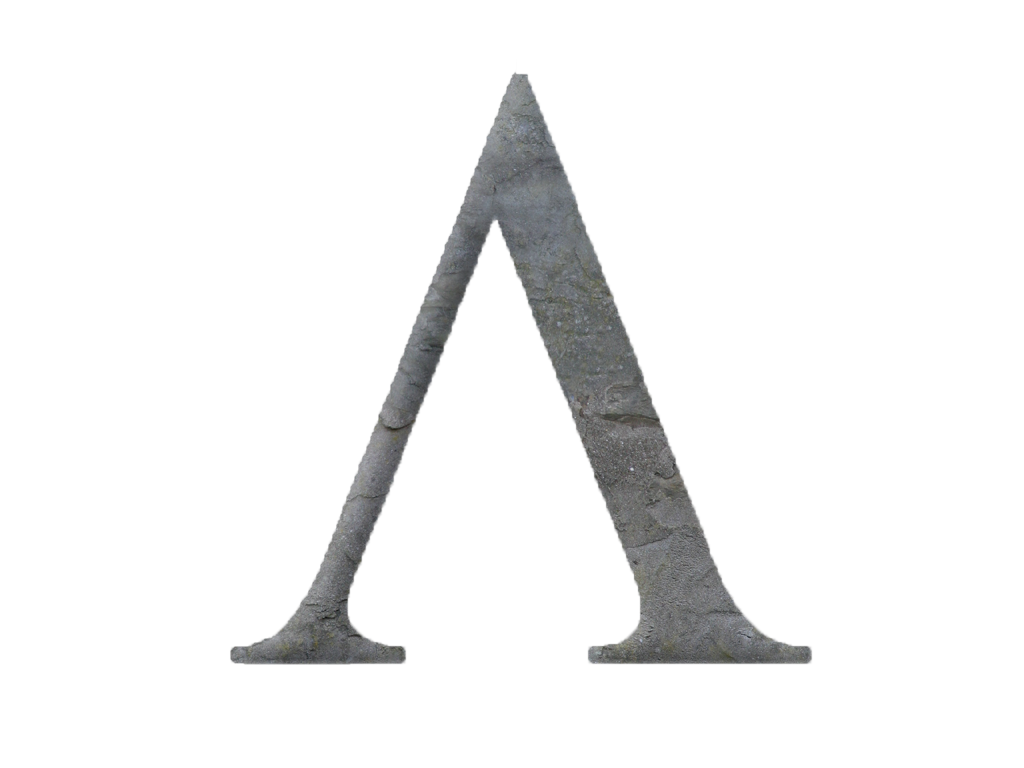
\includegraphics[width=1.0\paperwidth]{image/title-background.png}}

  \begin{frame}[plain] 
  \title{A note on your bravery}
  
  \vspace{3em}

  \begin{TitleBoxBravery}
    \begin{center}
    {\Large \inserttitle}
    \end{center}
  \end{TitleBoxBravery}

  \end{frame}
}


\begin{frame}
\frametitle{Introspection}
\begin{block}{So}
I typed ``functional programming for python'' into an internet search \ldots
\end{block}
\end{frame}


{
\usebackgroundtemplate{
\begin{tikzpicture}[remember picture,overlay]
  \coordinate (aa) at ($(a1)+(0,7.5)$);
  \node[right] at (aa) {
\includegraphics[height=1cm]{image/punch.jpg}};
\end{tikzpicture}
}


\begin{frame}
\frametitle{Bravery}
\begin{block}{Functional Programming \ldots}
The designers [of functional programming languages] \ldots choose to emphasize one particular approach to programming
\includegraphics[height=0.4cm]{image/bullshit.jpg} This is \ldots difficult to write programs that use a different approach
\includegraphics[height=0.4cm]{image/bullshit.jpg} Other languages are multi-paradigm languages that support several different approaches. Lisp, C++, and Python are multi-paradigm \ldots can write programs \ldots procedural, object-oriented, or functional in all of these languages
\includegraphics[height=0.4cm]{image/bullshit.jpg}
\end{block}
\end{frame}


\begin{frame}
\frametitle{Bravery}
\begin{block}{Some languages \ldots}
Some [functional programming] languages don't even have assignment statements such as \lstinline$a=3$ or \lstinline{c=a+b}
\includegraphics[height=0.4cm]{image/bullshit.jpg}, but it's difficult to avoid all side effects
\includegraphics[height=0.4cm]{image/bullshit.jpg} Printing to the screen or writing to a disk file are side effects, for example
\includegraphics[height=0.4cm]{image/bullshit.jpg}
\end{block}
\end{frame}


\begin{frame}
\frametitle{Bravery}
\begin{block}{Formal provability}
A theoretical benefit is that it’s easier to construct a mathematical proof that a functional program is correct
\includegraphics[height=0.4cm]{image/bullshit.jpg} \ldots Unfortunately, proving programs correct is largely impractical
\includegraphics[height=0.4cm]{image/bullshit.jpg} and not relevant to Python software
\includegraphics[height=0.4cm]{image/bullshit.jpg}
\end{block}
\end{frame}


\begin{frame}
\frametitle{Bravery}
\begin{block}{iterators}
a Python language feature that's an important foundation for writing functional-style programs: \textbf{iterators}
\includegraphics[height=0.4cm]{image/bullshit.jpg}
\end{block}
\end{frame}

}

{
\usebackgroundtemplate{
\begin{tikzpicture}[remember picture,overlay]
  \coordinate (aa) at ($(a1)+(0,7.5)$);
  \node[right] at (aa) {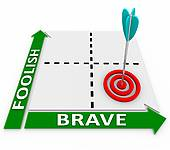
\includegraphics[height=2cm]{image/brave.jpg}};
\end{tikzpicture}
}

\begin{frame}
\frametitle{Introspection}
\begin{block}{Just when}
Just when I thought I'd seen enough, I realised \textbf{just how brave you all are}
\end{block}
\end{frame}

}